\documentclass[11pt,a4paper]{article}
\usepackage[margin=2.2cm]{geometry}
\usepackage{amsmath,amssymb,bm}
\usepackage{graphicx,float,booktabs,caption,subcaption}
\usepackage{xcolor}
\usepackage{listings}
\usepackage{tikz}
\usetikzlibrary{shapes.geometric,arrows.meta,positioning,calc}
\usepackage[colorlinks=true,linkcolor=blue!50!black,urlcolor=blue!50!black,citecolor=blue!50!black]{hyperref}
\usepackage{fancyhdr}
\pagestyle{fancy}\fancyhf{}\lhead{\small Karthick J (OE23S018), IIT Madras}\rhead{\small\leftmark}\cfoot{\thepage}
\definecolor{codebg}{rgb}{0.97,0.97,0.97}
\lstset{basicstyle=\ttfamily\scriptsize,backgroundcolor=\color{codebg},frame=single,breaklines=true,
 keywordstyle=\color{blue!60!black}\bfseries,commentstyle=\color{green!40!black},stringstyle=\color{red!50!black},
 numbers=left,numberstyle=\tiny\color{gray},showstringspaces=false,tabsize=4,columns=fullflexible,
 literate={²}{{$^2$}}1 {³}{{$^3$}}1 {°}{{$^\circ$}}1 {Δ}{{$\Delta$}}1 {ρ}{{$\rho$}}1 {μ}{{$\mu$}}1 {ω}{{$\omega$}}1 {ψ}{{$\psi$}}1 {α}{{$\alpha$}}1 {ν}{{$\nu$}}1 {τ}{{$\tau$}}1 {–}{{-}}1 {—}{{-}}1 {’}{{'}}1 {“}{{"}}1 {”}{{"}}1 {→}{{$\to$}}1 {≤}{{$\le$}}1 {≥}{{$\ge$}}1 {×}{{$\times$}}1 {±}{{$\pm$}}1 {·}{{$\cdot$}}1 {∂}{{$\partial$}}1 {∇}{{$\nabla$}}1 {γ}{{$\gamma$}}1 {ε}{{$\varepsilon$}}1 {μ}{{$\mu$}}1 {├}{{+}}1 {─}{{-}}1 {│}{{|}}1 {▶}{{>}}1 {▼}{{v}}1 {┌}{{+}}1 {┐}{{+}}1 {└}{{+}}1 {┘}{{+}}1 {┬}{{+}}1 {┴}{{+}}1}
\tikzset{
 startstop/.style={rectangle,rounded corners=6pt,minimum width=3.2cm,minimum height=0.8cm,text centered,draw=black,fill=red!12,font=\small},
 process/.style={rectangle,minimum width=4.6cm,minimum height=0.8cm,text centered,text width=5.6cm,draw=black,fill=blue!8,font=\small},
 decision/.style={diamond,aspect=2.6,text centered,text width=3.2cm,draw=black,fill=green!12,font=\small,inner sep=1pt},
 io/.style={trapezium,trapezium left angle=72,trapezium right angle=108,minimum width=3.6cm,minimum height=0.8cm,text centered,text width=4.6cm,draw=black,fill=orange!15,font=\small},
 arrow/.style={thick,-{Stealth[length=2.5mm]}}}
\setlength{\parskip}{4pt}\setlength{\parindent}{0pt}

\usepackage{longtable}
\title{\textbf{GPU-Accelerated Finite-Volume Simulation of Non-Newtonian Blood Flow in the Left Anterior Descending Artery}\\[2pt]\large Staggered-Grid Projection Method with QUICK Convection, Bird--Carreau Rheology and Block-Corrected SOR in CUDA C\\[2pt]\normalsize Course Project 1 -- OE5450 Numerical Techniques in Ocean Hydrodynamics (Final Project, Jan--May 2025)}
\author{Karthick J (OE23S018)\\Department of Ocean Engineering, IIT Madras}
\date{Revised report, October 2026}
\begin{document}\maketitle
\begin{abstract}
Steady laminar flow of blood, modelled as a shear-thinning Bird--Carreau fluid, is computed in a two-dimensional model of the proximal left anterior descending (LAD) coronary artery (length 140 mm, width 3.5 mm, mean velocity 0.39 m/s) with a finite-volume projection method on a staggered grid of $1400\times35$ cells. Every operation of the time step (boundary conditions, QUICK/central momentum predictor, divergence, pressure-correction sweeps, velocity correction, shear-rate and viscosity update, reductions) is a CUDA kernel. The submitted code did not compile; once it compiled, it produced NaN in the first time step. Twenty-five defects were corrected without changing the structure of the code; the most important were a pressure equation with the wrong sign that applied the pressure gradient twice, an outlet that was blocked because the last velocity face was never updated, walls moved one cell inwards, viscosity interpolated half a cell off, out-of-bounds QUICK stencils, an explicit time step 3.8 times the stability limit, and a pressure solver that cannot conserve mass on a 400:1 domain. The last point was fixed with a block (additive) correction along the artery, which reduced the mass error after the start-up from 4\% to $10^{-7}$ and the pressure-solver work four-fold. The kernels were verified by serial CPU emulation. In Newtonian mode the solver reproduces the exact solution of its discrete equations to $2.6\times10^{-6}$ and the Poiseuille pressure gradient to $0.12\%$; with Bird--Carreau rheology the developed velocity, shear-rate and viscosity profiles agree with an independent ODE solution within $0.2\%$, and the pressure gradient within $0.07\%$. Shear-thinning lowers the pressure drop over the 140 mm segment from 2994 Pa (Newtonian, $\mu_0$) to 335 Pa, flattens the core, and gives a wall shear stress of 4.2 Pa and a development length of 50 mm ($14W$).
\end{abstract}
\tableofcontents\newpage

\section{Problem definition}
\subsection{Physiological data}
The proximal LAD segment is represented, as in the original report, by a straight two-dimensional channel (Table~\ref{tab:par}). Blood is treated as an incompressible generalised Newtonian fluid of density $\rho$ whose apparent viscosity follows the Bird--Carreau law
\begin{equation}
\mu(\dot\gamma)=\mu_\infty+(\mu_0-\mu_\infty)\big[1+(\lambda\dot\gamma)^{a}\big]^{(n-1)/a},\qquad
\dot\gamma=\sqrt{2\Big(\frac{\partial u}{\partial x}\Big)^2+2\Big(\frac{\partial v}{\partial y}\Big)^2+\Big(\frac{\partial u}{\partial y}+\frac{\partial v}{\partial x}\Big)^2}, \label{eq:carreau}
\end{equation}
where $\dot\gamma$ is the shear rate (second invariant of the rate-of-strain tensor).
\begin{table}[H]\centering\small
\resizebox{\textwidth}{!}{\begin{tabular}{llll}\toprule
Quantity & Symbol & Value & Note\\\midrule
length, width & $L$, $W$ & 0.14 m, 3.5 mm & proximal LAD (Ali et al.\ 2024)\\
mean inflow velocity & $U$ & 0.39 m/s & time-averaged; inlet profile $1.5U(1-\eta^2)$\\
density & $\rho$ & 1060 kg/m$^3$ &\\
Carreau parameters & $\mu_0,\mu_\infty,\lambda,n,a$ & 0.056 Pa\,s, 0.0035 Pa\,s, 3.13 s, 0.6, 2 & original report$^\dagger$\\
grid & $N_x\times N_y$ & $1400\times35$, $\Delta x=\Delta y=0.1$ mm & 49\,000 cells\\
Reynolds number & $\rho UW/\mu$ & 25.8 ($\mu_0$), 245 ($\mu_w$), 413 ($\mu_\infty$) & $\mu_w$: developed wall value\\\bottomrule
\end{tabular}}\caption{Parameters. $^\dagger$The widely used fit of Cho \& Kensey (1991) has $\mu_\infty=0.00345$ Pa\,s, $\lambda=3.313$ s, $n=0.3568$; the values of the original project are kept here.}\label{tab:par}\end{table}

\subsection{Governing equations and boundary conditions}
\begin{align}
\nabla\cdot\mathbf{u}&=0,\\
\rho\Big(\frac{\partial\mathbf{u}}{\partial t}+\nabla\cdot(\mathbf{u}\mathbf{u})\Big)&=-\nabla p+\nabla\cdot\big(\mu(\dot\gamma)\nabla\mathbf{u}\big). \label{eq:mom}
\end{align}
The viscous term is used in the Laplacian form of the original code. For variable viscosity the full stress divergence contains in addition $\nabla\cdot(\mu\nabla\mathbf{u}^T)=(\nabla\mu)\cdot(\nabla\mathbf{u})^T$; this term vanishes identically in fully developed flow ($v=0$, $\partial u/\partial x=0$) and is small in the gently developing entrance flow considered here, so it was kept as a documented modelling simplification rather than changed.

Boundary conditions: parabolic inflow $u=1.5U(1-\eta^2)$, $v=0$ at $x=0$ ($\eta=2y/W-1$); no slip at $y=0,W$; at $x=L$ zero streamwise gradient of $u$, $v=0$ in the last cell column and fixed pressure $p=0$. The fluid is initially at rest with a linear pressure field $p=\Delta P(1-x/L)$, $\Delta P=2886.3$ Pa (the original Poiseuille estimate); the steady state is reached by time marching.

\section{Numerical method}
\subsection{Staggered finite-volume grid}
Pressure, viscosity and shear rate are stored at cell centres $(i,j)$; $u_{i,j}$ on the west face of cell $i$ ($i=0\ldots N_x$, index \texttt{i+j*(nx+1)}) and $v_{i,j}$ on the south face of cell $j$ ($j=0\ldots N_y$, index \texttt{i+j*nx}). Each velocity component has its own control volume centred on its face (Fig.~\ref{fig:grid}). No-slip on the walls is imposed through antisymmetric ghost values, $u_{i,-1}=-u_{i,0}$, $u_{i,N_y}=-u_{i,N_y-1}$, so that the wall lies exactly on $y=0$ and $y=W$.
\begin{figure}[H]\centering
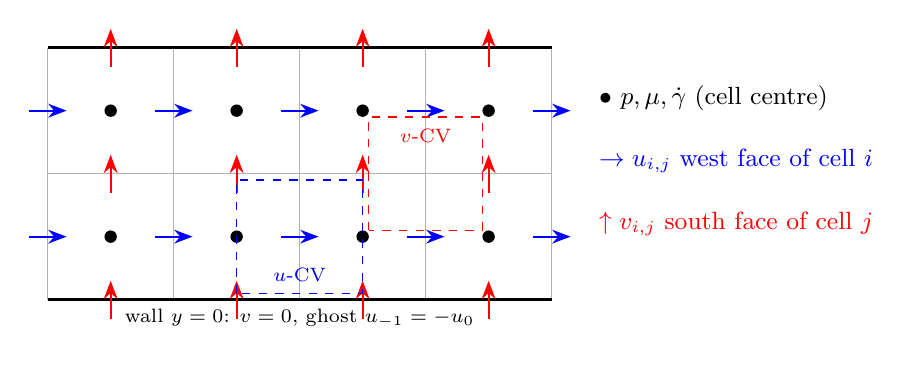
\begin{tikzpicture}[scale=1.6]
\draw[gray!60](0,0)grid(4,2); \draw[very thick](0,0)--(4,0);\draw[very thick](0,2)--(4,2);
\foreach \i in {0,1,2,3}\foreach \j in {0,1}{\fill(\i+0.5,\j+0.5)circle(1.4pt);}
\foreach \i in {0,1,2,3,4}\foreach \j in {0,1}{\draw[-{Stealth},blue,thick](\i-0.15,\j+0.5)--(\i+0.15,\j+0.5);}
\foreach \i in {0,1,2,3}\foreach \j in {0,1,2}{\draw[-{Stealth},red,thick](\i+0.5,\j-0.15)--(\i+0.5,\j+0.15);}
\draw[dashed,blue](1.5,0.05)rectangle(2.5,0.95); \node[blue,font=\scriptsize] at (2.0,0.2){$u$-CV};
\draw[dashed,red](2.55,0.55)rectangle(3.45,1.45); \node[red,font=\scriptsize] at (3.0,1.3){$v$-CV};
\node[font=\scriptsize,below] at (2,0){wall $y=0$: $v=0$, ghost $u_{-1}=-u_0$};
\node[right,font=\small] at (4.3,1.6){$\bullet$ $p,\mu,\dot\gamma$ (cell centre)};
\node[right,font=\small,blue] at (4.3,1.1){$\rightarrow u_{i,j}$ west face of cell $i$};
\node[right,font=\small,red] at (4.3,0.6){$\uparrow v_{i,j}$ south face of cell $j$};
\end{tikzpicture}
\caption{MAC arrangement near the lower wall and the two momentum control volumes. Faces of the $u$-CV lie at cell centres (east/west) and at cell corners (north/south); this determines where viscosity and transverse velocity must be interpolated.}\label{fig:grid}\end{figure}

\subsection{Momentum predictor}
Explicit Euler with the pressure of the previous step gives the intermediate velocity, e.g.\ for the $u$-CV of face $(i,j)$:
\begin{multline}
u^*_{ij}=u^n_{ij}+\frac{\Delta t}{\Delta x\Delta y}\Big[-(F_e\phi_e-F_w\phi_w+F_n\phi_n-F_s\phi_s)\\+\frac{D_e(u_E-u_P)-D_w(u_P-u_W)+D_n(u_N-u_P)-D_s(u_P-u_S)}{\rho}\Big]-\frac{\Delta t}{\rho}\frac{p_{ij}-p_{i-1,j}}{\Delta x},
\end{multline}
with volume fluxes $F_e=\tfrac12(u_P+u_E)\Delta y$, $F_n=\tfrac12(v_{i-1,j+1}+v_{i,j+1})\Delta x$ (two-point averages on the CV faces), diffusion conductances $D_e=\mu_e\Delta y/\Delta x$, $D_n=\mu_n\Delta x/\Delta y$ with $\mu_e=\mu_{i,j}$, $\mu_w=\mu_{i-1,j}$ (cell centres) and $\mu_{n},\mu_s$ the four-cell averages at the corners. Face values $\phi_f$ use QUICK (Leonard 1979),
\begin{equation}
\phi_f=\tfrac68\phi_U+\tfrac38\phi_D-\tfrac18\phi_{UU},
\end{equation}
($U$ upstream, $D$ downstream, $UU$ far upstream of the face, chosen by the sign of $F_f$), and first-order upwind where $UU$ would lie outside the domain (first interior faces). The $v$-equation is analogous.

\subsection{Pressure correction (projection)}
Writing $\mathbf{u}^{n+1}=\mathbf{u}^*-(\Delta t/\rho)\nabla p'$ and requiring $\nabla\cdot\mathbf{u}^{n+1}=0$ gives, cell by cell,
\begin{equation}
\sum_{nb}a_{nb}\,(p'_{nb}-p'_P)=\frac{\rho}{\Delta t}\,(\nabla\cdot\mathbf{u}^*)_P,\qquad a_{E,W}=\frac1{\Delta x^2},\;a_{N,S}=\frac1{\Delta y^2}, \label{eq:pp}
\end{equation}
with $a_{nb}=0$ across faces whose velocity is not corrected (inlet face, walls, $v$-faces of the inlet column), i.e.\ $\partial p'/\partial n=0$ there, and $p'=0$ in the outlet column. Then $u^{n+1}=u^*-(\Delta t/\rho)\,\delta_xp'$, $v^{n+1}=v^*-(\Delta t/\rho)\,\delta_yp'$ and $p^{n+1}=p^n+p'$ (incremental projection). Because the predictor already contains $\nabla p^n$, the zero initial guess for $p'$ is equivalent to a warm start $p^{n+1}=p^n$, and $p'\to0$ at steady state, where the converged solution satisfies the discrete momentum and continuity equations exactly. Eq.~\eqref{eq:pp} is solved by red--black SOR ($\omega=1.85$) until the mean change per sweep is below $10^{-6}$ Pa.

\paragraph{Why point SOR alone fails on an artery-shaped domain.} The slowest error mode of Eq.~\eqref{eq:pp} is uniform across the channel and varies over the whole length (Neumann inlet, Dirichlet outlet): wavenumber $\theta_x=\pi/(2N_x)$, Jacobi spectral radius $\rho_J=(1+\cos\theta_x)/2\approx1-\theta_x^2/4=1-3.1\times10^{-7}$. For SOR with $\omega$ below the optimum of this mode the eigenvalue is $1-\delta$ with $\delta=2\omega\epsilon/(2-\omega)$, $\epsilon=1-\rho_J$: $\delta=6\epsilon=1.9\times10^{-6}$ per sweep for the original $\omega=1.5$. Even 1000 sweeps per step therefore reduce this mode by only $0.2\%$. Physically it is the cross-sectional flow rate $Q(x)$: without a converged correction, mass is not conserved along the artery (Section~\ref{sec:ablation}).

\paragraph{Block correction.} Following Settari \& Aziz (1973) and Patankar (1980), every ten sweeps a constant $c_i$ is added to all cells of column $i$ such that the column-summed residual $R_i=\sum_j r_{ij}$ of Eq.~\eqref{eq:pp} vanishes. Summing Eq.~\eqref{eq:pp} over a column, the north/south terms cancel and
\begin{equation}
A_W\,c_{i-1}-(A_W+A_E)\,c_i+A_E\,c_{i+1}=R_i,\qquad A_E=A_W=\frac{N_y}{\Delta x^2}\;(A_W=0\text{ at the inlet}),\quad c_{N_x-1}=0,
\end{equation}
a tridiagonal system solved by the Thomas algorithm. For this separable operator the correction removes the cross-sectionally uniform component of the error exactly, leaving modes with $\theta_y\ge\pi/N_y$, for which $\rho_J\le0.998$ and $\omega_{opt}=2/(1+\sin(\pi/N_y))\approx1.84$; this is why $\omega=1.85$ was chosen. The result is that every cross-section carries exactly the inflow, and the solver converges in 17--25 sweeps per step.

\subsection{Explicit stability limit}
For explicit Euler with central/QUICK fluxes, Fourier analysis of the linearised predictor gives two conditions. For the highest wavenumber ($\theta=\pi$ in both directions) the amplification factor is $G=1-8d-\sigma_Q$ with $d=\nu\Delta t/\Delta x^2$ and $\sigma_Q$ the QUICK (upwind-biased) contribution $\approx$ CFL; $|G|\le1$ requires
\begin{equation}
\Delta t\le\Big[\frac{|u|}{\Delta x}+\frac{|v|}{\Delta y}+\frac{2\mu}{\rho}\Big(\frac1{\Delta x^2}+\frac1{\Delta y^2}\Big)\Big]^{-1}. \label{eq:dt1}
\end{equation}
For low wavenumbers the forward-Euler central convection must be damped by diffusion, $|G|^2\approx1+(\sigma^2-2d)\theta^2$, which requires
\begin{equation}
\Delta t\le\frac{2\mu}{\rho|\mathbf{u}|^2}. \label{eq:dt2}
\end{equation}
Both are evaluated cell by cell (with the local $\mu$) by a reduction kernel and applied with a safety factor 0.9, together with CFL $\le0.5$ and a growth limit of 1.5 per step. With $\mu=\mu_0$ on the centreline Eq.~\eqref{eq:dt1} gives $\Delta t=3.34\times10^{-5}$ s. The original step, $0.5\Delta x/U=1.28\times10^{-4}$ s, is 3.8 times larger. Even the pure diffusion limit $\rho\Delta x^2/(4\mu_0)=4.7\times10^{-5}$ s is not sufficient: a run at that value developed a sustained cell-to-cell oscillation at the outlet with velocities of 1.1 m/s.

\subsection{CUDA implementation}
\begin{table}[H]\centering\small
\begin{tabular}{p{4.1cm}p{3.3cm}p{7.6cm}}\toprule
Kernel & threads & work per thread\\\midrule
\texttt{ApplyBoundaryConditions} & $(N_x+1)(N_y+1)$ & inlet profile, outlet $\partial u/\partial x=0$, $p_{out}$, wall $v=0$\\
\texttt{Xmomentum\_solver} & one per $u$-face & QUICK fluxes, face viscosities, predictor $u^*$\\
\texttt{YMomentum\_solver} & one per $v$-face & same for $v^*$\\
\texttt{Divergence} & one per cell & $(\nabla\cdot\mathbf{u}^*)_P$\\
\texttt{PoissonSolverGS} (2 launches) & one per cell, red / black & SOR update of $p'$; \texttt{atomicAdd} of $|\delta p'|$\\
\texttt{ColumnResidual} & one per column & $R_i=\sum_j r_{ij}$ (35 cells)\\
\texttt{BlockCorrectionTDMA} & 1 & Thomas algorithm, 1399 unknowns\\
\texttt{ApplyBlockCorrection} & one per cell & $p'_{ij}\mathrel{+}=c_i$\\
\texttt{CorrectVelocities} & one per face/cell & projection, $p\mathrel{+}=p'$\\
\texttt{Shear\_rate} & one per cell & $\dot\gamma$ with ghost values, Bird--Carreau $\mu$\\
\texttt{CalculateResidual}, \texttt{CalculateMaxVelocity} & one per face/cell & \texttt{atomicAdd}/\texttt{atomicMax} reductions for convergence and $\Delta t$\\\bottomrule
\end{tabular}\caption{Kernels ($16\times16$ thread blocks; the launch grid covers $(N_x+1)\times(N_y+1)$ so that the outlet and top-wall faces have threads).}\end{table}
All kernels except the SOR sweep write to arrays they do not read (Jacobi-style), and the SOR sweep is split into red and black half-sweeps, so there are no data races. Float reductions use \texttt{atomicMax} on the integer image of non-negative floats, which preserves ordering. Each array holds $\approx$0.2 MB, so the whole state ($\approx$3 MB) fits in the L2 cache of a modern GPU; the cost per step is dominated by kernel-launch and synchronisation overhead of the 2 launches and one host copy per SOR sweep.

\paragraph{Verification without a GPU.} The workspace used for this revision has no GPU. The kernels were executed by \texttt{tools/cuda\_cpu\_shim.h}: \texttt{tools/emulate.sh} rewrites every launch \texttt{k<<<G,B>>>(args)} into a loop over \texttt{blockIdx}/\texttt{threadIdx} that calls the unmodified kernel once per thread, and maps the runtime API (\texttt{cudaMalloc}, \texttt{cudaMemcpy}, \texttt{cudaMemset}, events, \texttt{atomicAdd}, \texttt{atomicMax}, \texttt{\_\_float\_as\_int}) to host equivalents. Because no kernel has a data race, the serial execution reproduces the GPU result up to the summation order of the atomic adds. \texttt{run.sh} compiles the same file with \texttt{nvcc} and repeats the runs on the GPU when one is present.

\subsection{Algorithm}
\begin{figure}[H]\centering
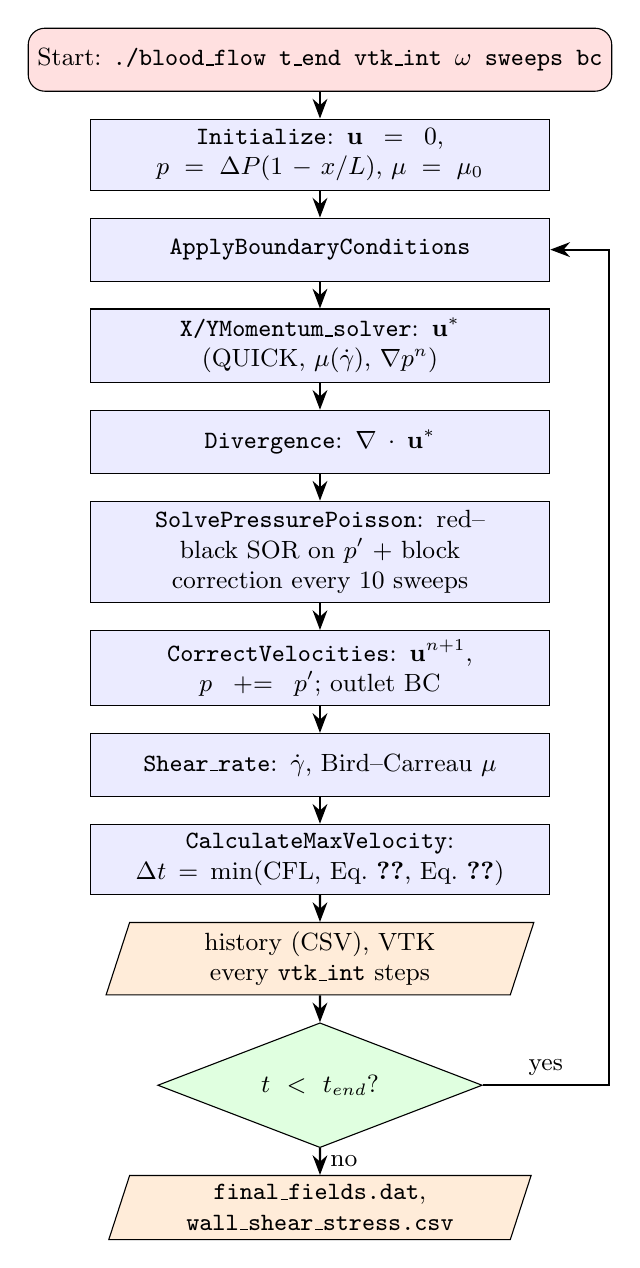
\begin{tikzpicture}[node distance=0.34cm]
\node(s)[startstop]{Start: \texttt{./blood\_flow t\_end vtk\_int $\omega$ sweeps bc}};
\node(i)[process,below=of s]{\texttt{Initialize}: $\mathbf{u}=0$, $p=\Delta P(1-x/L)$, $\mu=\mu_0$};
\node(b)[process,below=of i]{\texttt{ApplyBoundaryConditions}};
\node(m)[process,below=of b]{\texttt{X/YMomentum\_solver}: $\mathbf{u}^*$ (QUICK, $\mu(\dot\gamma)$, $\nabla p^n$)};
\node(dv)[process,below=of m]{\texttt{Divergence}: $\nabla\cdot\mathbf{u}^*$};
\node(pp)[process,below=of dv]{\texttt{SolvePressurePoisson}: red--black SOR on $p'$ + block correction every 10 sweeps};
\node(c)[process,below=of pp]{\texttt{CorrectVelocities}: $\mathbf{u}^{n+1}$, $p\mathrel{+}=p'$; outlet BC};
\node(sr)[process,below=of c]{\texttt{Shear\_rate}: $\dot\gamma$, Bird--Carreau $\mu$};
\node(dt)[process,below=of sr]{\texttt{CalculateMaxVelocity}: $\Delta t=\min$(CFL, Eq.~\ref{eq:dt1}, Eq.~\ref{eq:dt2})};
\node(o)[io,below=of dt]{history (CSV), VTK every \texttt{vtk\_int} steps};
\node(d)[decision,below=of o]{$t<t_{end}$?};
\node(f)[io,below=of d]{\texttt{final\_fields.dat}, \texttt{wall\_shear\_stress.csv}};
\draw[arrow](s)--(i);\draw[arrow](i)--(b);\draw[arrow](b)--(m);\draw[arrow](m)--(dv);\draw[arrow](dv)--(pp);\draw[arrow](pp)--(c);\draw[arrow](c)--(sr);\draw[arrow](sr)--(dt);\draw[arrow](dt)--(o);\draw[arrow](o)--(d);
\draw[arrow](d)--node[right,font=\small]{no}(f);
\draw[arrow](d.east)--node[above,font=\small]{yes}++(1.6,0)|-(b.east);
\end{tikzpicture}\caption{Time step of \texttt{code/Blood\_flow.cu}; all boxes except I/O are CUDA kernels.}\end{figure}

\section{Code review of the submitted program}
The submitted file is kept as \texttt{original/Blood\_flow\_original.cu} (the CPU port and the listing printed in the report are kept alongside). It does not compile: kernel parameters named \texttt{dt}, \texttt{DX}, \texttt{DY}, \texttt{rho} are replaced by the macros of the same name, and two prototypes contain \texttt{int 1401, int 36}. With only these compile errors removed (\texttt{original/Blood\_flow\_original\_compile\_fixes\_only.cu}) the program runs but the residual is NaN from the first step and the pressure is NaN in 47\,600 of the 49\,000 cells after 1.3 ms (\texttt{original/run\_of\_original\_compile\_fixed\_only\_log.txt}). The original report contains no simulation results, so there are no earlier plots to compare with. The errors and corrections (marked \texttt{[FIX]} in \texttt{code/Blood\_flow.cu}) are:
{\small
\begin{longtable}{p{3.5cm}p{11.7cm}}\toprule
Location & Error $\rightarrow$ correction\\\midrule\endhead
prototypes, kernel parameters & Macro/parameter name clashes and numeric parameter names: did not compile $\rightarrow$ renamed \texttt{dt\_val}, \texttt{dx}, \texttt{dy}, \texttt{rho\_val}.\\
\texttt{NX}, \texttt{NY} & \texttt{(int)(L/DX)+1} counts nodes, but the arrays hold cells: $1401\times36$ cells = $140.1\times3.6$ mm $\rightarrow$ rounded cell counts $1400\times35$.\\
inlet profile & $\eta=2j/(N_y-1)-1$ puts zero velocity in the first and last fluid rows (cell centres), and $U(1-\eta^2)$ has mean $2U/3=0.26$ m/s instead of the stated mean 0.39 m/s $\rightarrow$ $\eta=2(j+\frac12)/N_y-1$, $1.5U(1-\eta^2)$.\\
inlet pressure & $p_0=p_1$ imposed every step removes the pressure force on face 1 $\rightarrow$ removed; inlet condition enters the pressure-correction equation.\\
wall rows of $u$ & $u=0$ imposed on rows $j=0$ and $N_y-1$, which lie inside the fluid: walls moved one cell inwards (33 fluid rows) $\rightarrow$ ghost-cell no-slip.\\
momentum ranges & $u$ solved for $1\le i<N_x-1$, $1\le j<N_y-1$: face $N_x-1$ never updated, so the outlet face kept $u=0$ and \emph{blocked the channel}; wall rows frozen. $v$ solved for $j<N_y-1$ $\rightarrow$ all interior faces.\\
uninitialised $\mathbf{u}^*$ & boundary faces of $u^*,v^*$ never written (raw \texttt{cudaMalloc} memory) but read by \texttt{Divergence} and \texttt{CorrectVelocities} $\rightarrow$ copied from $\mathbf{u}^n$.\\
QUICK stencil & reads $u_{i-2}$ at $i=1$ and $u_{j\pm2}$ next to the walls: out-of-bounds memory $\rightarrow$ upwind where the far-upstream node does not exist.\\
transverse velocity on CV faces & four-point averages give $v$ (resp.\ $u$) at the CV centre and were used for both faces $\rightarrow$ two-point face averages.\\
face viscosities & averaged with the wrong neighbours (half a cell off) $\rightarrow$ cell values on east/west faces, four-cell corner averages on north/south faces.\\
shear rate & cross derivatives were one-sided (at $y_{j+1/2}$); wall-adjacent and inlet/outlet cells were given $\mu=\mu_0$, the \emph{largest} viscosity where the shear rate is largest $\rightarrow$ central differences with ghost values in all cells.\\
divergence & computed for interior cells only; boundary-cell entries uninitialised $\rightarrow$ all cells.\\
pressure equation sign & source $-\rho\nabla\cdot\mathbf{u}^*/\Delta t$ has the wrong sign for $\mathbf{u}=\mathbf{u}^*-(\Delta t/\rho)\nabla p'$ $\rightarrow$ $+$.\\
pressure equation $\Delta t$ & used the macro $\Delta t=10^{-5}$ s, not the adaptive step taken $\rightarrow$ actual $\Delta t$.\\
pressure unknown & solved for the full $p$ although the predictor already contains $\nabla p$, then corrected with $\nabla p$ again (pressure counted twice) $\rightarrow$ incremental correction $p'$, $p\mathrel{+}=p'$.\\
SOR race & all cells updated in one launch while reading neighbours from the array being written (non-deterministic Jacobi/Gauss--Seidel mix) $\rightarrow$ red--black ordering.\\
pressure BCs & boundary cells never updated in the solver $\rightarrow$ Neumann (walls, inlet) / Dirichlet (outlet) built into the coefficients.\\
mass conservation & point SOR cannot correct the axial flow rate on a $1400\times35$ domain (Section~2.3) $\rightarrow$ block correction.\\
``SIMPLE'' loop & each of up to 1000 inner passes re-predicted from the current $\mathbf{u}$ with the full $\Delta t$, i.e.\ advanced the flow by another step while the clock advanced once $\rightarrow$ one predictor--projection per step (explicit fractional-step method).\\
time step & CFL step $1.28\times10^{-4}$ s is 3.8 times the stability limit $\rightarrow$ Eqs.~\eqref{eq:dt1}--\eqref{eq:dt2}; growth limiter \texttt{fminf(dt,1.5*dt)} was a no-op $\rightarrow$ limits growth relative to the previous step; final step split to avoid a $\sim$\,ns step.\\
residual kernel & loop bounds missed the outlet faces and the top wall row $\rightarrow$ all faces; reported as RMS $\partial u/\partial t$.\\
memory management & \texttt{cudaMalloc}/\texttt{cudaFree} inside the time loop and inside every pressure solve $\rightarrow$ allocated once.\\
launch grid & sized by $N_x,N_y$, covering the $N_x+1$ / $N_y+1$ faces only by accident $\rightarrow$ $(N_x+1)\times(N_y+1)$.\\
VTK output & \texttt{DIMENSIONS} counts points; writing $N_x\times N_y$ points dropped the last cell row and column $\rightarrow$ $(N_x+1)\times(N_y+1)$; viscosity and shear rate added.\\
input & interactive \texttt{scanf} $\rightarrow$ command-line arguments (batch runs).\\\bottomrule
\end{longtable}}

\section{Verification: Newtonian Poiseuille flow}
With $\lambda=0$ the Carreau law reduces to a Newtonian fluid with $\mu=\mu_0$. For this case the exact solution of the \emph{discrete} equations is known: substituting $u_j=\frac{G}{2\mu}y_j(W-y_j)+c$ into the five-point operator with the ghost condition $u_{-1}=-u_0$ gives $c=Gh^2/(8\mu)$, and the flow-rate constraint then gives $G_{disc}=12\mu\bar U_d/[W^2(1+2/N_y^2)]$, where $\bar U_d=1.000408\,U$ is the midpoint-rule mean of the sampled inlet parabola. A 20 mm channel was run to $t=0.3$ s ($13$ viscous time constants $W^2/\pi^2\nu$).
\begin{figure}[H]\centering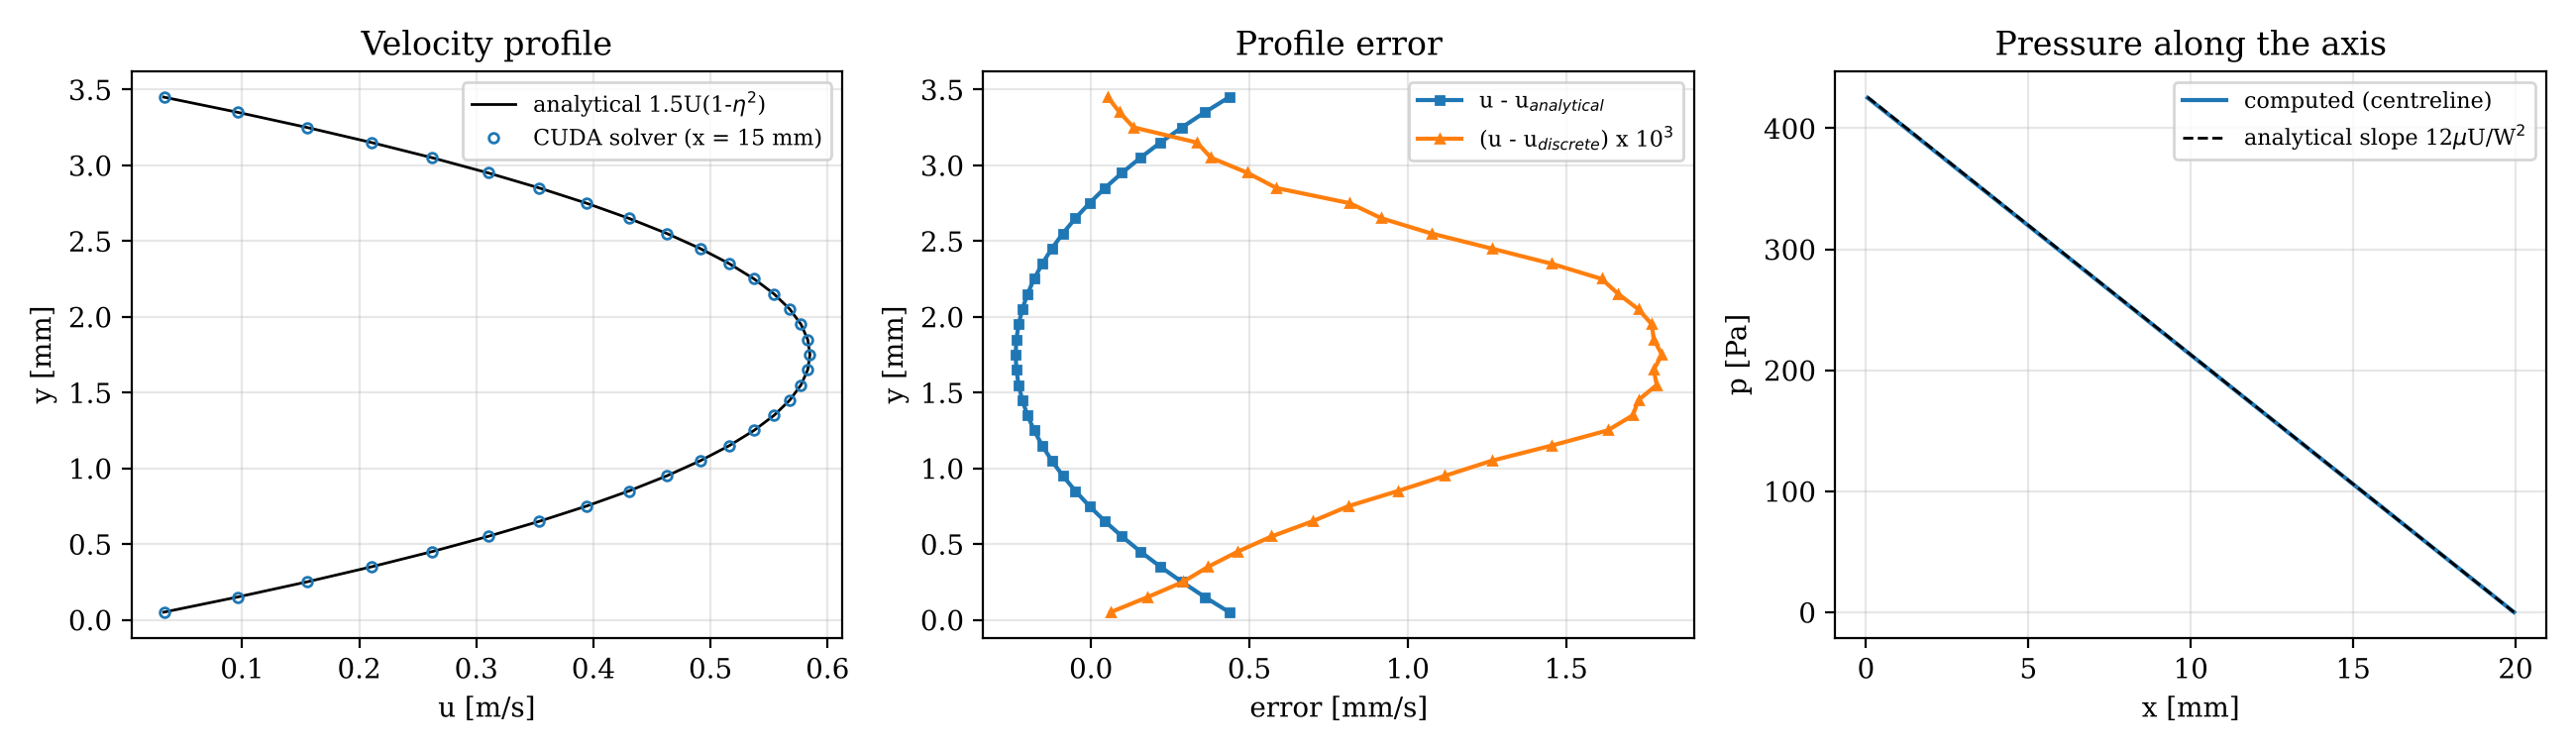
\includegraphics[width=\textwidth]{../results/fig7_newtonian_verification.png}
\caption{Newtonian verification at $x=15$ mm: profile, error relative to the analytical and to the exact discrete solution, and axial pressure.}\end{figure}
\begin{table}[H]\centering\small
\begin{tabular}{lccc}\toprule
Quantity & computed & analytical (rel.\ error) & exact discrete (rel.\ error)\\\midrule
$G=-dp/dx$ [Pa/m] & 21\,368.08 & 21\,394.29 ($-1.2\times10^{-3}$) & 21\,368.13 ($-2.6\times10^{-6}$)\\
$\max|u-u_{ref}|$ [m/s] & -- & $4.4\times10^{-4}$ (0.075\% of $u_{max}$) & $1.8\times10^{-6}$\\
$\tau_w$ [Pa] & 37.394 & 37.440 ($-1.2\times10^{-3}$) & --\\\bottomrule
\end{tabular}\caption{Newtonian verification.}\end{table}
The solver reproduces its own exact discrete solution to single-precision round-off, which verifies the momentum predictor, the projection, the pressure boundary conditions and the ghost-cell walls; the remaining difference from the analytical solution is the expected $O(h^2)$ discretisation error ($2/N_y^2=0.16\%$ in $G$).

\section{Results: Bird--Carreau flow in the LAD}
The full domain was integrated to $t=2$ s ($59\,961$ steps, 5.6 flow-through times $L/U$, 9 viscous time constants based on $\mu_w$).

\subsection{Convergence and mass conservation}
\begin{figure}[H]\centering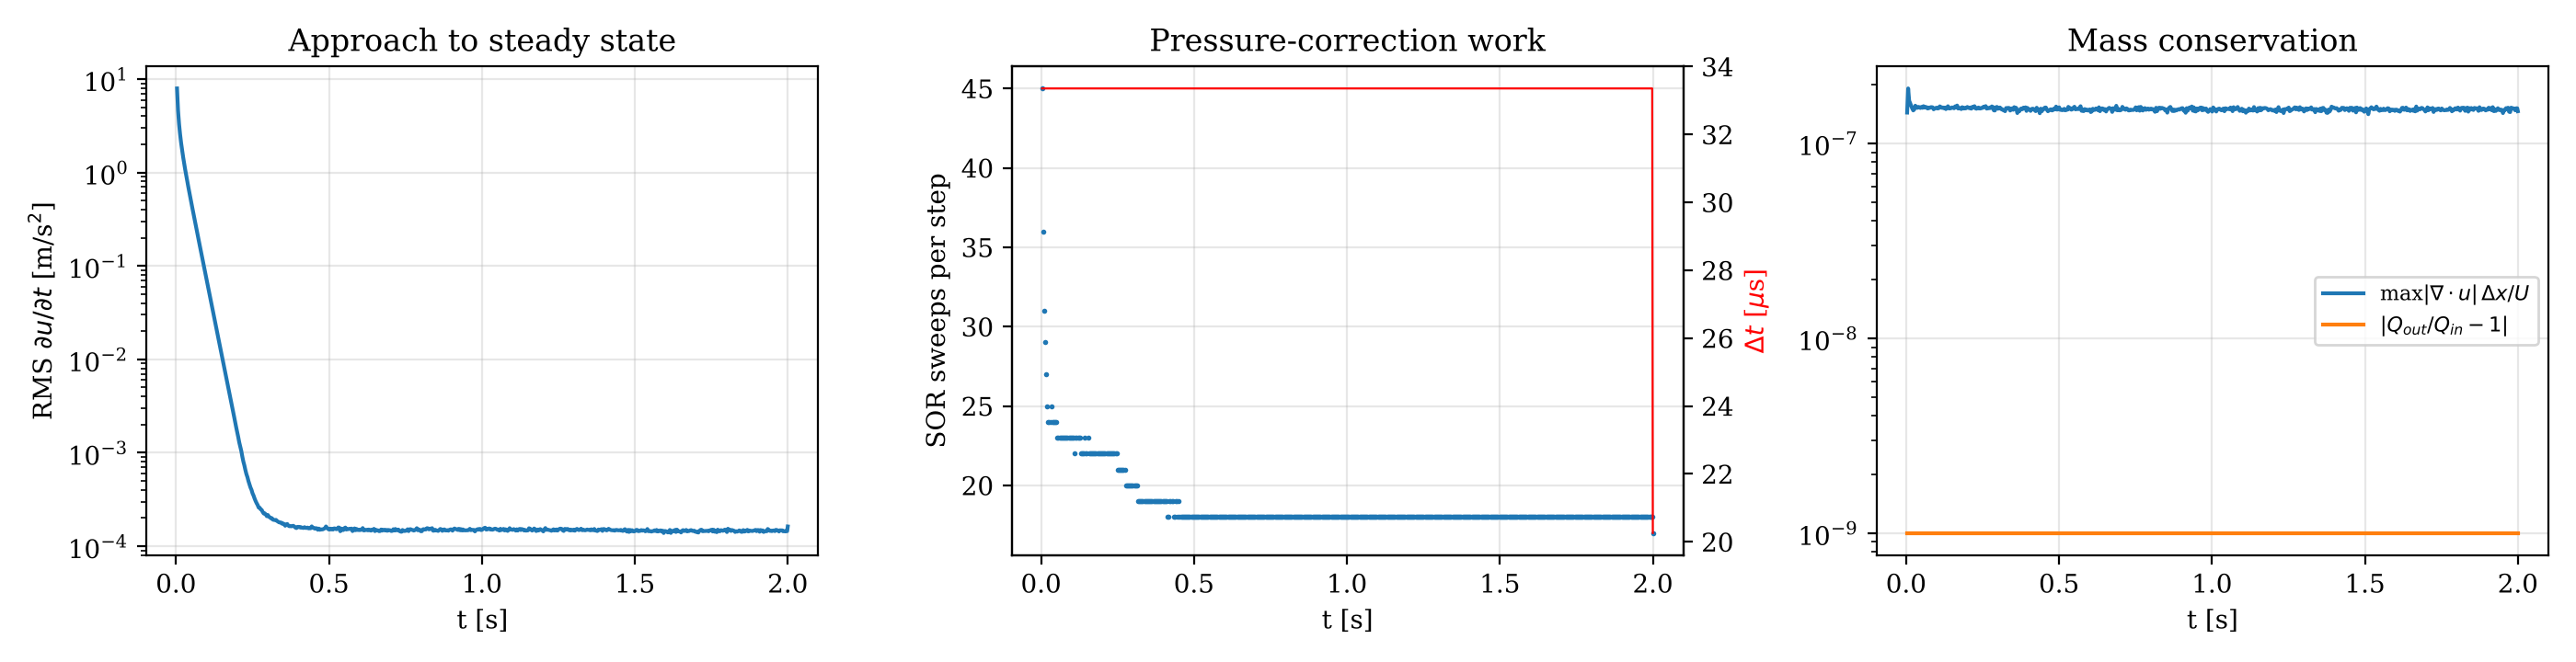
\includegraphics[width=\textwidth]{../results/fig6_convergence.png}
\caption{RMS $\partial u/\partial t$, SOR sweeps per step and time step, and mass-conservation errors.}\end{figure}
The RMS rate of change falls by five orders of magnitude within 0.3 s and then stays at $1.5\times10^{-4}$ m/s$^2$, which corresponds to a change of $5\times10^{-9}$ m/s per step, the single-precision round-off level. The pressure solver needs 45 sweeps per step at start-up and 18 at steady state. The divergence after projection is $\le1.9\times10^{-7}U/\Delta x$ and the outflow equals the inflow to round-off throughout.

\subsection{Flow field}
\begin{figure}[H]\centering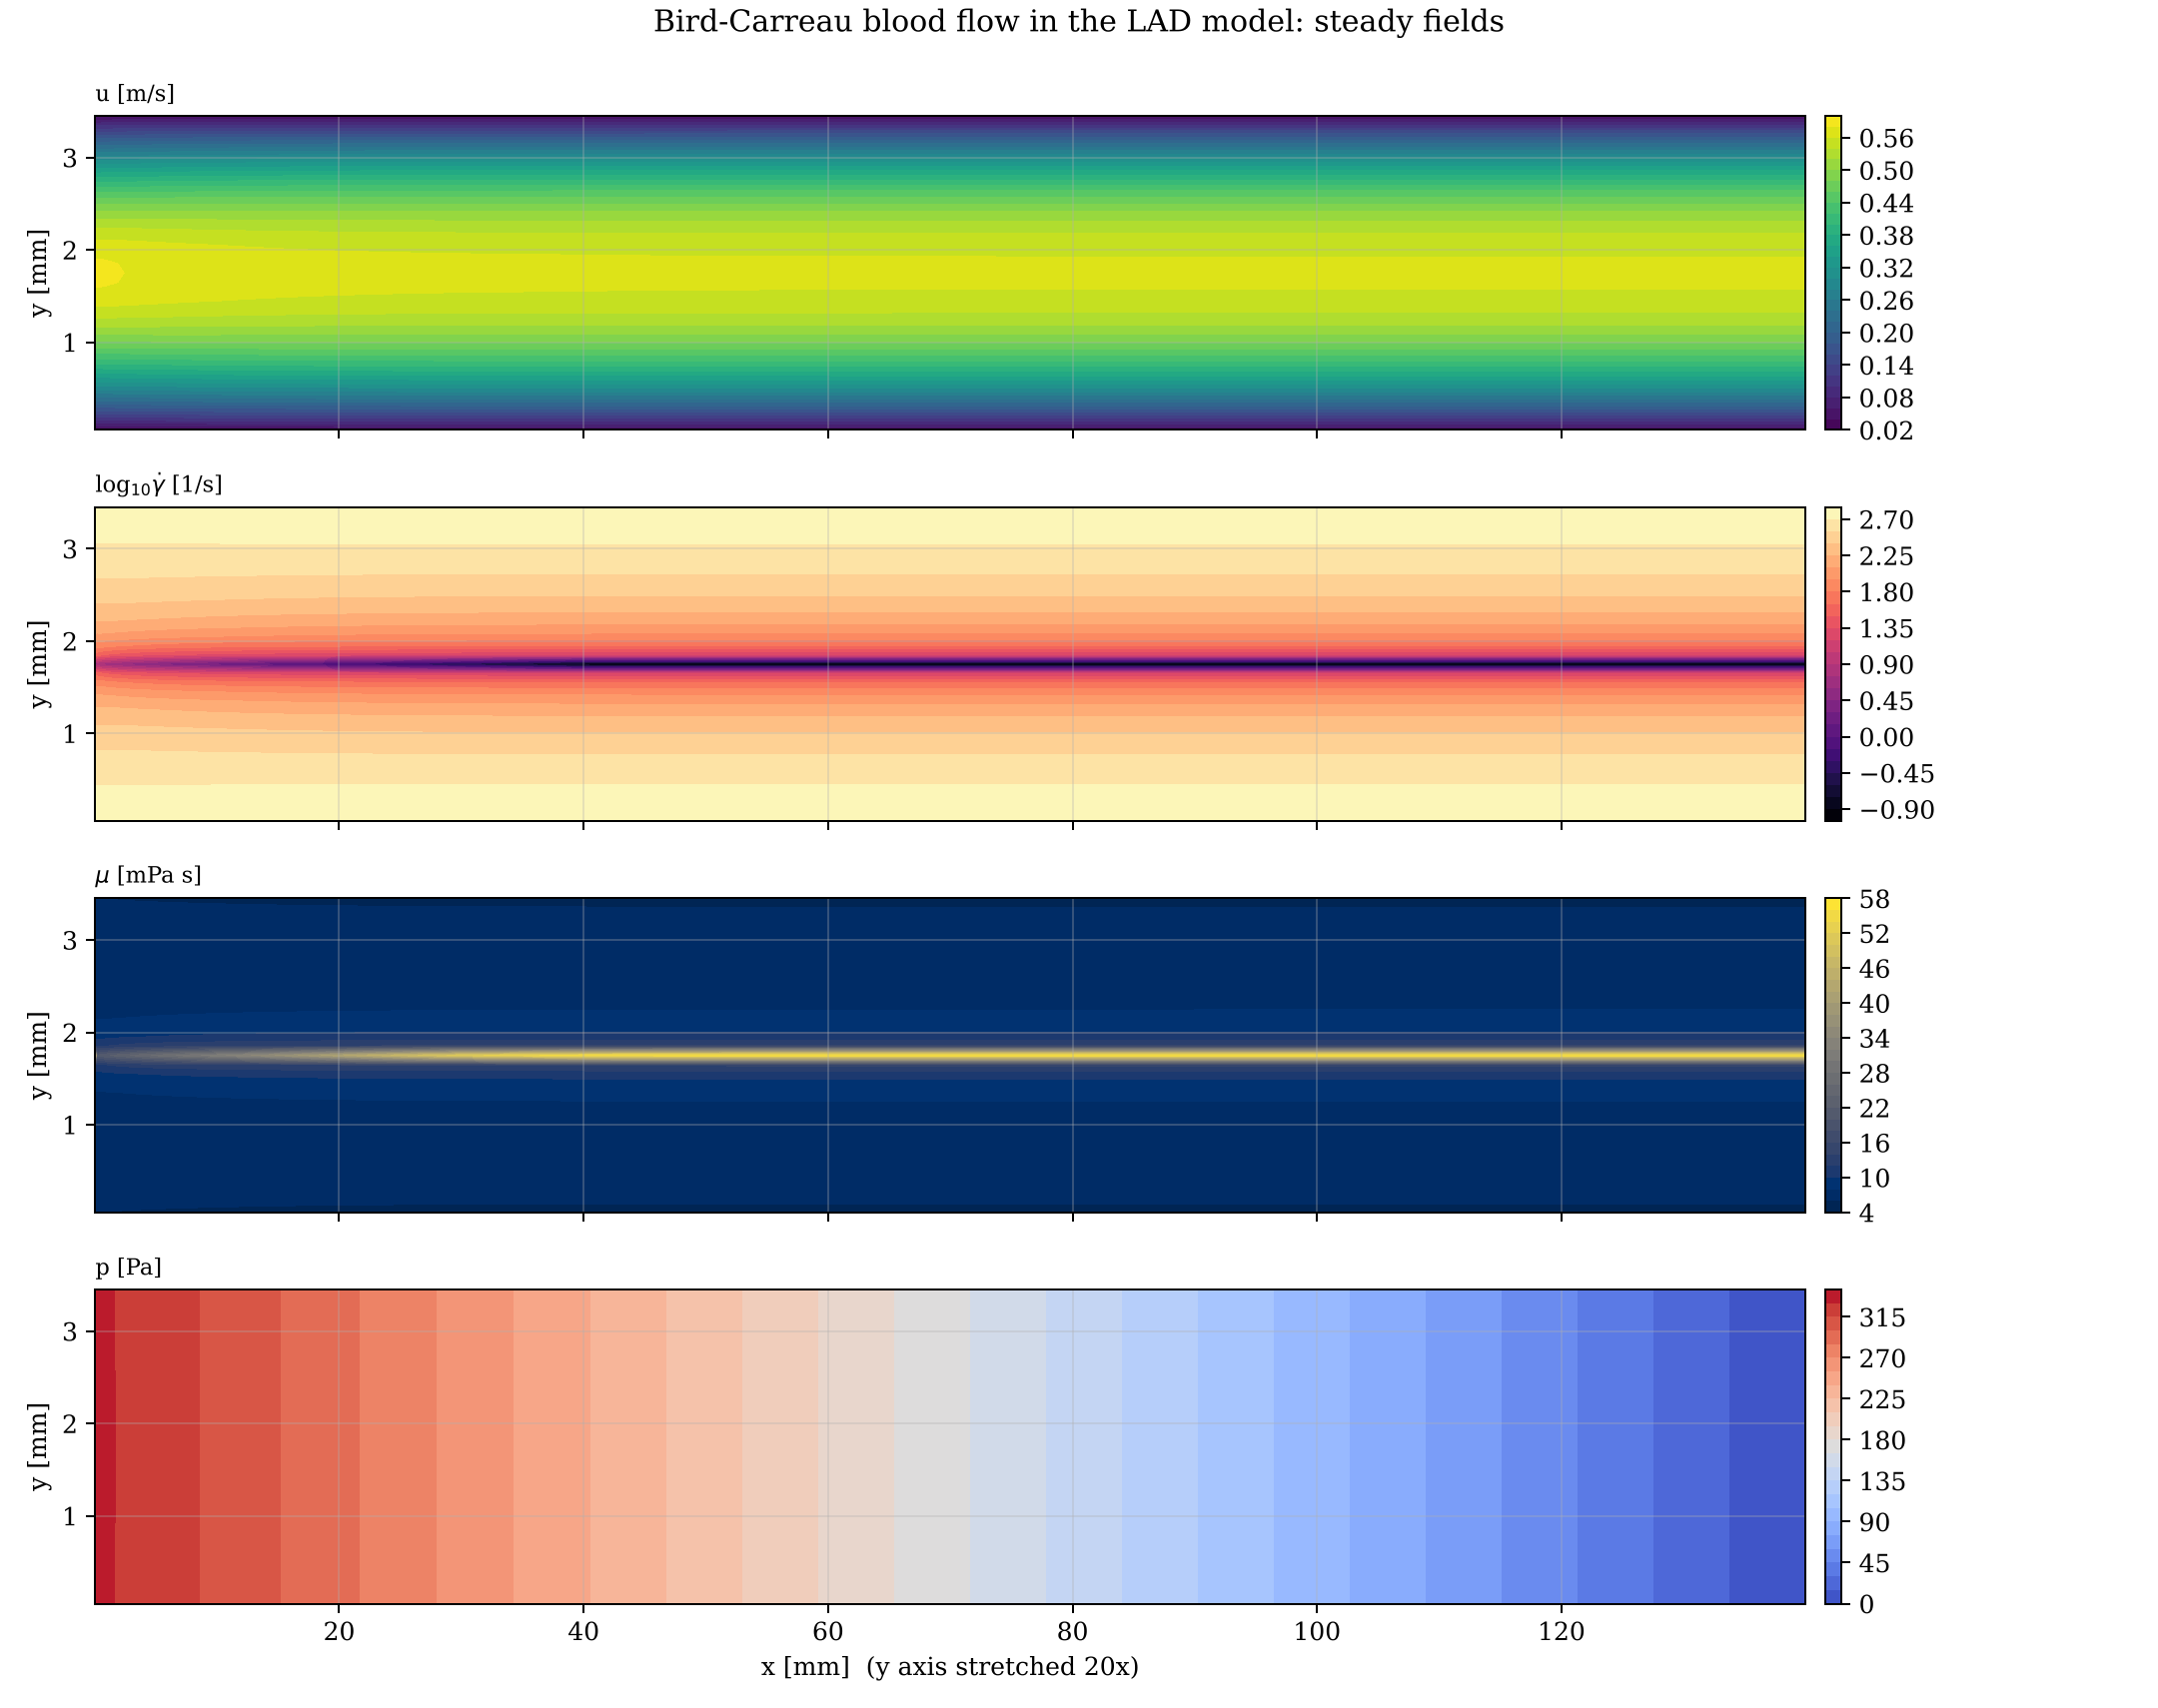
\includegraphics[width=\textwidth]{../results/fig1_fields.png}
\caption{Steady $u$, shear rate, viscosity and pressure (the $y$ axis is stretched 20 times).}\end{figure}
\begin{figure}[H]\centering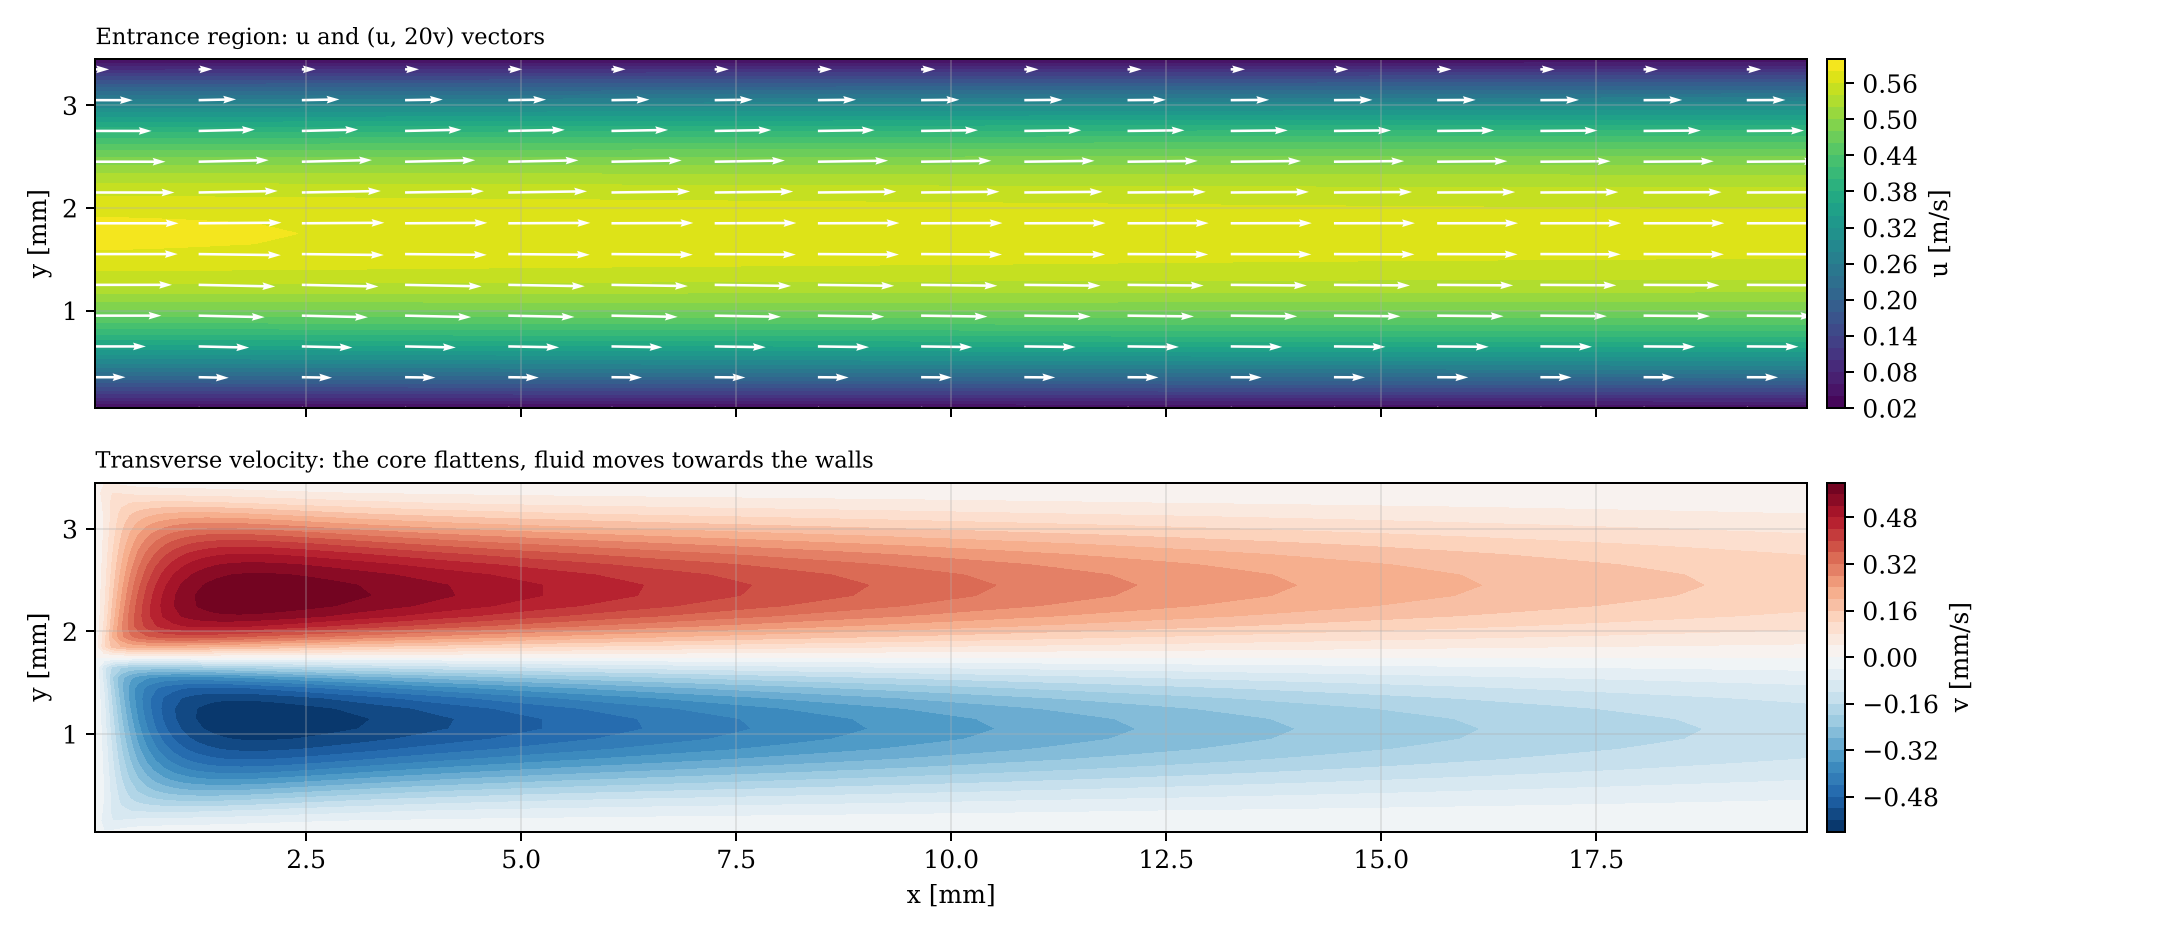
\includegraphics[width=\textwidth]{../results/fig2_entrance_region.png}
\caption{Entrance region: the parabolic inflow is blunted by shear-thinning; the transverse velocity (up to 0.6 mm/s) carries fluid from the core towards the walls.}\end{figure}
Shear-thinning concentrates the viscosity in a thin core around the centreline, where $\dot\gamma\to0$ and $\mu\to\mu_0=56$ mPa\,s, while over most of the section $\dot\gamma=10^2$--$7\times10^2$ s$^{-1}$ and $\mu=6$--$10$ mPa\,s. The parabolic inflow (the Newtonian developed profile) is therefore not an equilibrium profile: the core decelerates, the near-wall fluid accelerates, and the transverse velocity of Fig.~2 redistributes the flow until the developed Carreau profile is reached.

\subsection{Developed flow: comparison with the exact Carreau solution}
For fully developed flow, $d(\mu\dot\gamma)/ds=-G$ gives $\mu(\dot\gamma)\dot\gamma=Gs$ ($s$ = distance from the centreline), which is inverted for $\dot\gamma(s)$ (monotone because $n>0$) and integrated, $u(s)=\int_s^{W/2}\dot\gamma\,ds'$; $G$ follows from $\frac{2}{W}\int_0^{W/2}u\,ds=\bar U_d$ (bisection, 4001 points, \texttt{code/postprocess.py}).
\begin{figure}[H]\centering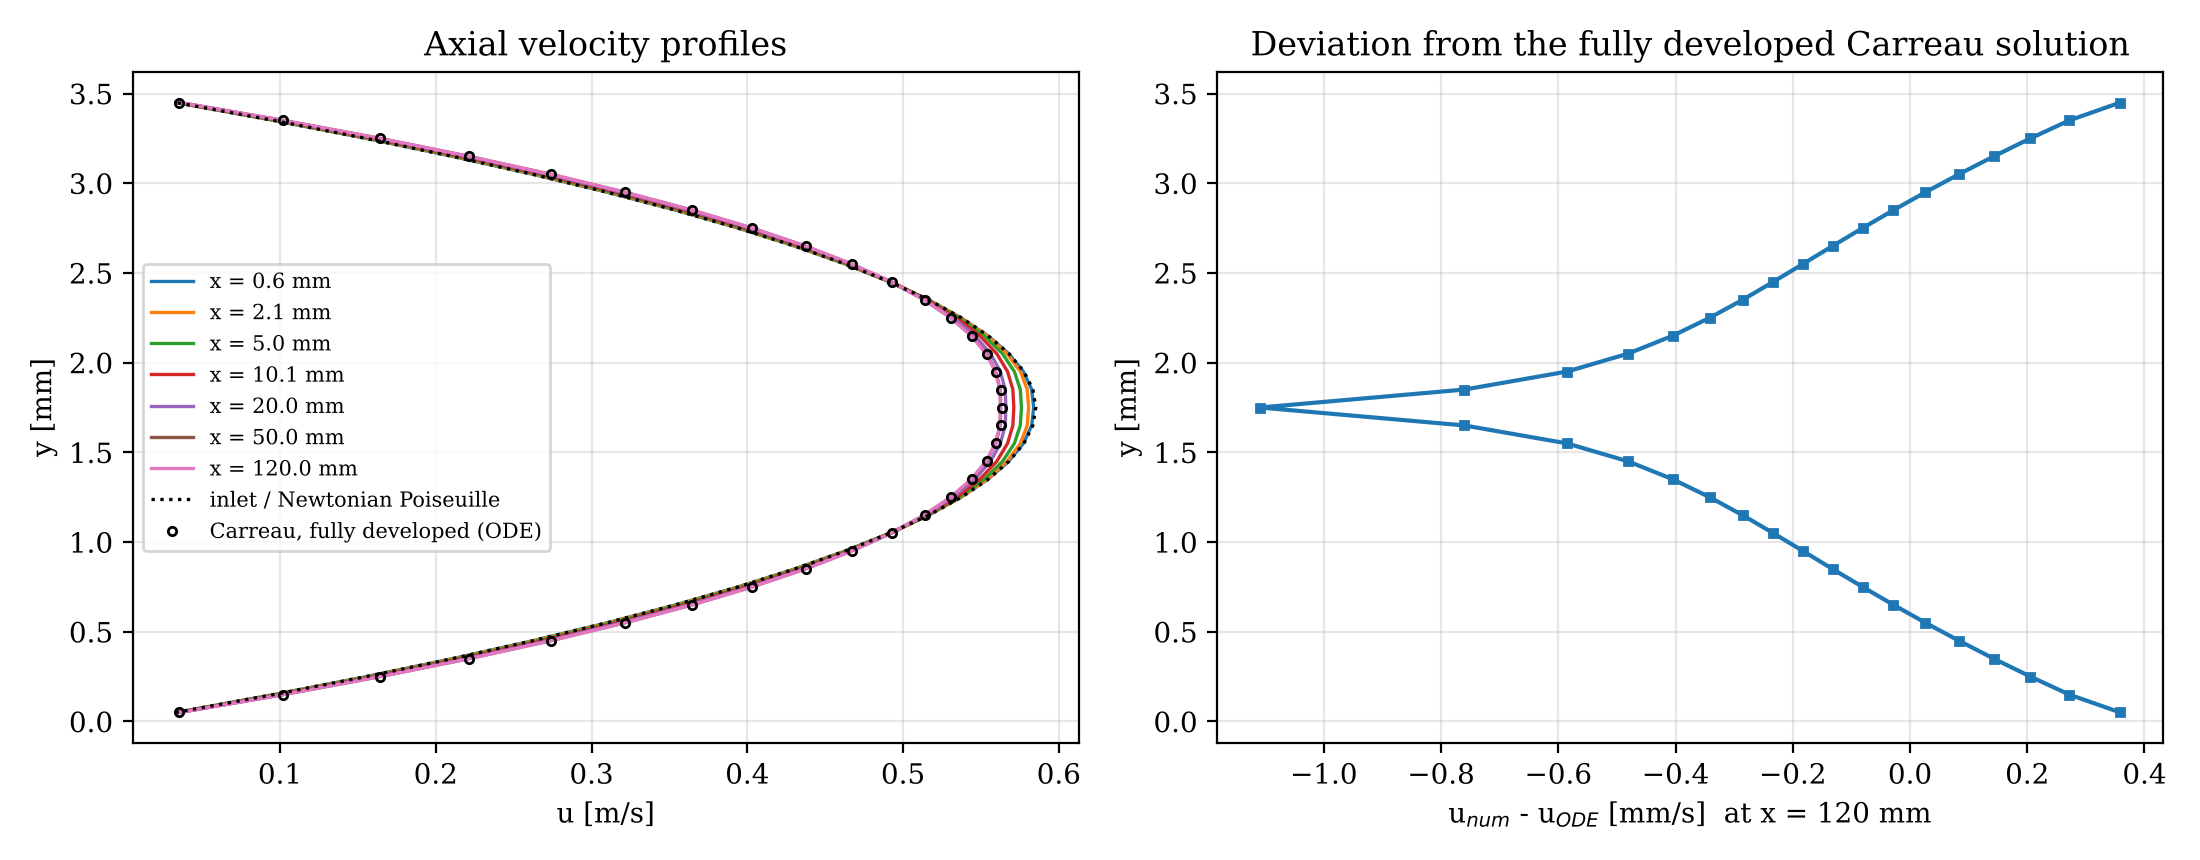
\includegraphics[width=\textwidth]{../results/fig3_profiles.png}
\caption{Velocity profiles along the artery and deviation from the exact developed Carreau profile at $x=120$ mm.}\end{figure}
\begin{figure}[H]\centering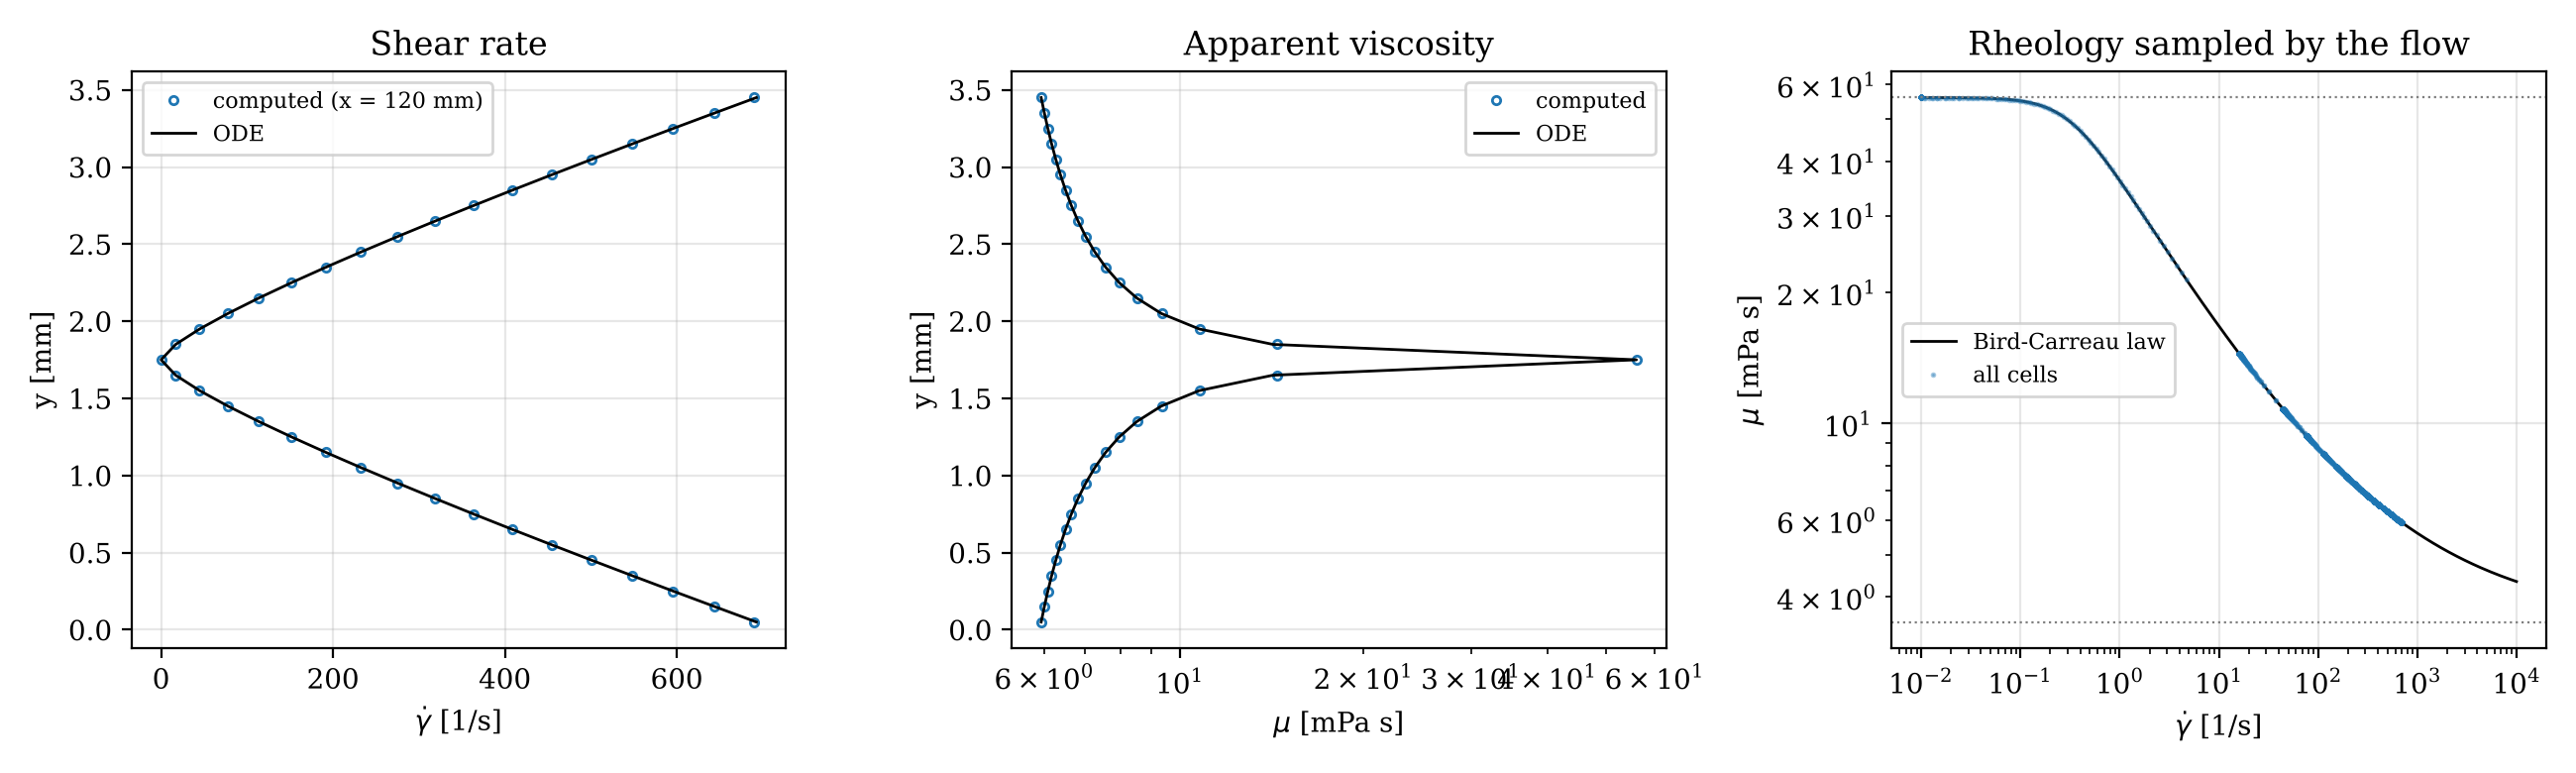
\includegraphics[width=\textwidth]{../results/fig5_shear_viscosity.png}
\caption{Shear rate and viscosity across the developed section against the ODE, and the part of the Carreau curve sampled by the flow.}\end{figure}
\begin{table}[H]\centering\small
\resizebox{\textwidth}{!}{\begin{tabular}{lccc}\toprule
Quantity & computed & exact developed (rel.\ error) & Newtonian $\mu_0$ / $\mu_\infty$\\\midrule
$G=-dp/dx$ [Pa/m] ($x>80$ mm) & 2414.4 & 2416.2 ($-7.4\times10^{-4}$) & 21\,403 / 1338\\
centreline velocity [m/s] & 0.5625 & 0.5636 ($-0.20\%$) & 0.585 / 0.585\\
$\max|u-u_{ODE}|$ [m/s] & $1.1\times10^{-3}$ & (0.20\% of $u_c$) & --\\
wall shear stress $\tau_w$ [Pa] & 4.204 & 4.228 ($-0.59\%$) & 37.46 / 2.34\\
wall shear rate [s$^{-1}$], wall viscosity [mPa\,s] & -- & 717, 5.90 & 669, 56 / 3.5\\
pressure drop over the segment [Pa] & 334.7 & 338.0 ($G\,(L-\Delta x)$) & 2994 / 187\\
development length $L_e$ (1\% criterion) & 50.4 mm $=14.4W$ & -- & --\\\bottomrule
\end{tabular}}\caption{Developed-flow quantities. The largest local error (0.2\%) is in the centreline cell, where $\mu$ varies by a factor of five within one cell.}\end{table}

\subsection{Pressure and wall shear stress along the artery}
\begin{figure}[H]\centering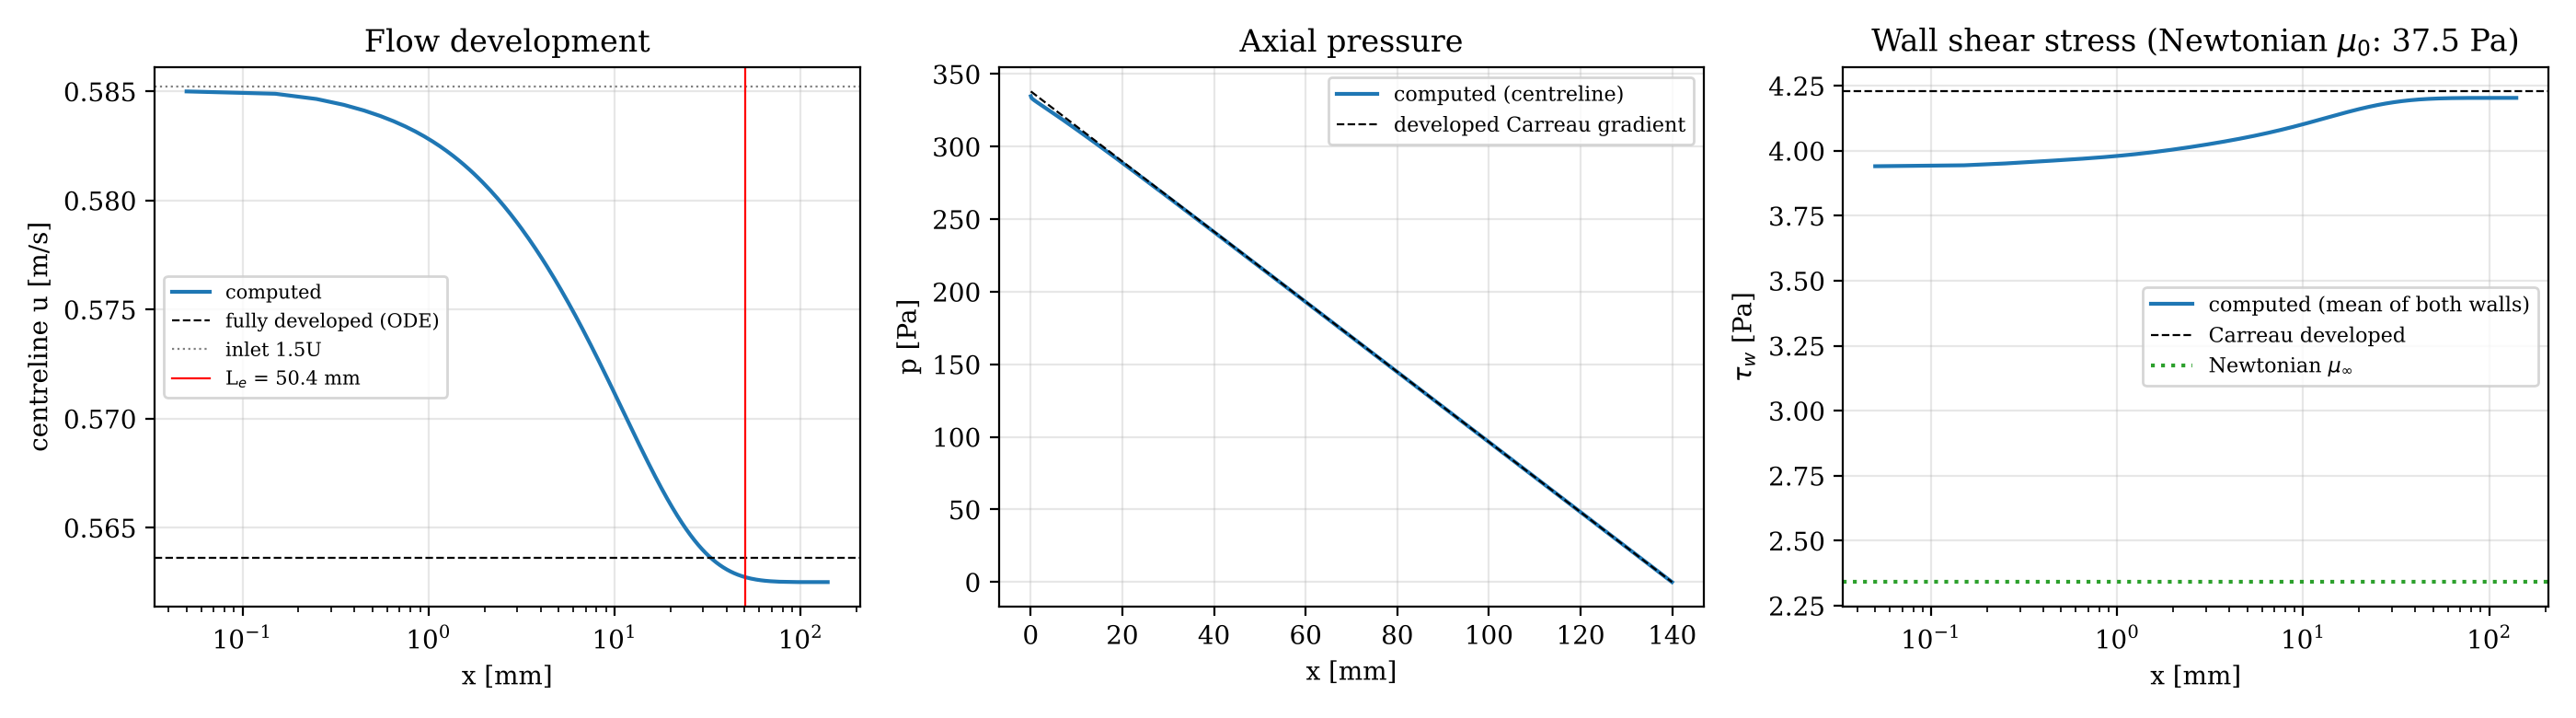
\includegraphics[width=\textwidth]{../results/fig4_development_pressure_wss.png}
\caption{Centreline velocity, axial pressure and wall shear stress.}\end{figure}
The pressure falls linearly after the entrance region, with the developed Carreau gradient. The wall shear stress rises from 3.94 Pa at the inlet (parabolic profile with $\mu$ evaluated at the Newtonian wall shear rate) to the developed value 4.20 Pa as the profile blunts and the wall shear rate increases from 669 to 717 s$^{-1}$. A Newtonian model with the zero-shear viscosity would overpredict the pressure drop and the wall shear stress by a factor of nine; the high-shear-limit model underpredicts them by 45\%. Since WSS in the range 1--7 Pa is the physiological reference for coronary arteries, the choice of rheological model is not a detail.

\subsection{Block correction: effect on mass conservation and cost}\label{sec:ablation}
\begin{figure}[H]\centering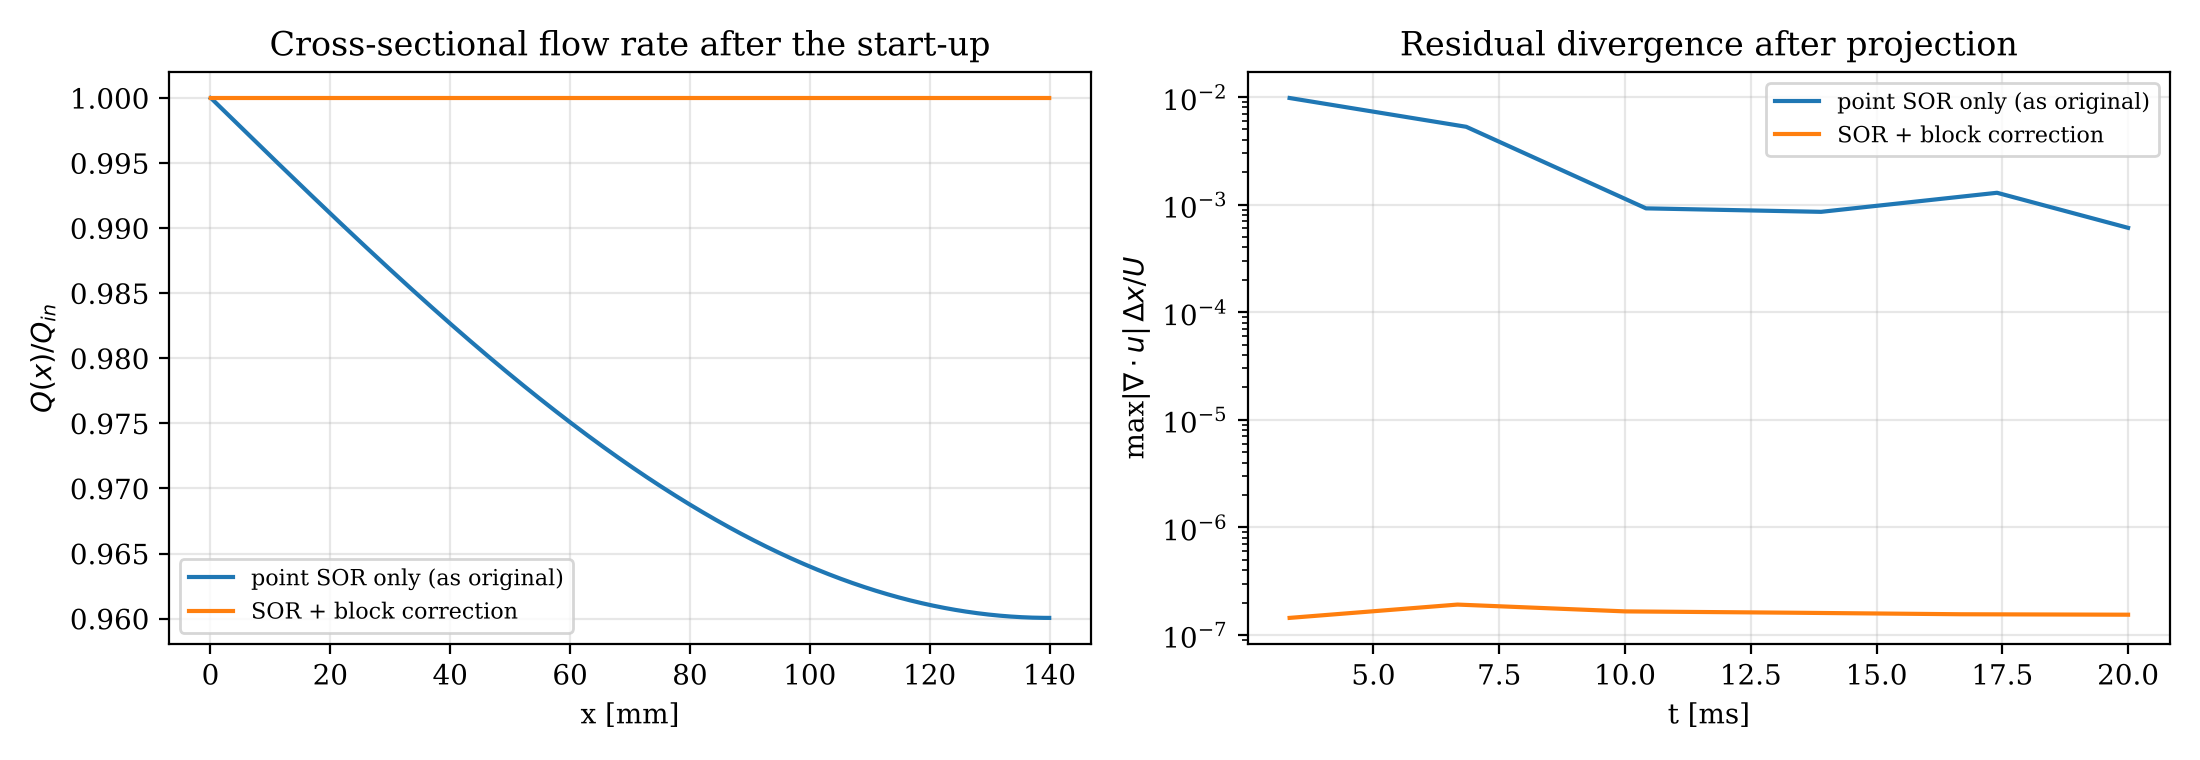
\includegraphics[width=\textwidth]{../results/fig8_block_correction.png}
\caption{First 20 ms of the full case with point SOR only (1000 sweeps per step, as the original) and with the block correction.}\end{figure}
With point SOR every step uses the maximum of 1000 sweeps, the residual divergence stays at $6\times10^{-4}U/\Delta x$, and after 20 ms only 96\% of the inflow leaves the artery. With the block correction each cross-section carries the inflow to round-off, the solver converges in about 25 sweeps, and the run is 4.3 times faster (58.6 against 252.9 ms per step in the emulation).

\subsection{Run time}
The complete $t=2$ s run takes 612 s in the serial CPU emulation (10.2 ms per step, 49\,000 cells, about 18 SOR sweeps per step), the Newtonian check 24 s. On a GPU the cost per step is dominated by the $\approx$50 kernel launches and the per-sweep host copy of the convergence residual; \texttt{run.sh} records the GPU times in \texttt{results/timing.txt}. Checking the residual every few sweeps, fusing the red and black half-sweeps into one launch with shared-memory tiles, and moving the reductions to warp-level primitives are the natural next optimisations.

\section{Limitations}
\begin{itemize}
\item The artery is a straight two-dimensional channel (planar Poiseuille base flow), not an axisymmetric or patient-specific tube; curvature, branches, stenoses and wall motion are not modelled.
\item The inflow is steady (time-averaged velocity); coronary flow is pulsatile, with a Womersley number of order 2--3.
\item The viscous term uses the Laplacian form $\nabla\cdot(\mu\nabla\mathbf{u})$ of the original code; the omitted $\nabla\cdot(\mu\nabla\mathbf{u}^T)$ vanishes in developed flow.
\item Single precision limits the steady residual to $\sim10^{-4}$ m/s$^2$, which is adequate for the quantities reported.
\end{itemize}

\section{Conclusions}
\begin{itemize}
\item The submitted CUDA finite-volume code did not compile, and with compile errors removed it produced NaN in the first step. Twenty-five defects (listed in Section~3) were corrected while keeping the kernels and the data layout; the pressure-correction solver was extended with a block correction, without which point SOR cannot conserve mass along a 400:1 artery.
\item In Newtonian mode the solver reproduces the exact solution of its discrete equations to $2.6\times10^{-6}$ (single-precision round-off) and the analytical Poiseuille gradient to $0.12\%$.
\item With Bird--Carreau rheology the developed velocity, shear-rate and viscosity profiles agree with the exact solution within $0.2\%$ and the pressure gradient within $0.07\%$. Shear-thinning blunts the profile (centreline velocity $1.44\bar U$ instead of $1.5\bar U$), develops over 50 mm ($14W$), and gives $\tau_w=4.2$ Pa and a pressure drop of 335 Pa over the 140 mm segment.
\end{itemize}

\section*{References}
\small
S.\ Ali et al., Journal of X-Ray Science and Technology (2024) -- LAD geometry and mean velocity (as cited in the original report).\\
Y.I.\ Cho, K.R.\ Kensey, Effects of the non-Newtonian viscosity of blood on flows in a diseased arterial vessel, \emph{Biorheology} 28 (1991) 241--262.\\
B.P.\ Leonard, A stable and accurate convective modelling procedure based on quadratic upstream interpolation, \emph{Comput.\ Methods Appl.\ Mech.\ Eng.} 19 (1979) 59--98.\\
A.J.\ Chorin, Numerical solution of the Navier--Stokes equations, \emph{Math.\ Comp.} 22 (1968) 745--762.\\
F.H.\ Harlow, J.E.\ Welch, \emph{Phys.\ Fluids} 8 (1965) 2182--2189 (MAC grid).\\
A.\ Settari, K.\ Aziz, A generalization of the additive correction methods for the iterative solution of matrix equations, \emph{SIAM J.\ Numer.\ Anal.} 10 (1973) 506--521.\\
S.V.\ Patankar, \emph{Numerical Heat Transfer and Fluid Flow}, Hemisphere, 1980.\\
NVIDIA, \emph{CUDA C++ Programming Guide}.
\normalsize
\section*{Reproducing the results}
\texttt{bash run.sh} builds \texttt{code/Blood\_flow.cu}, runs the cases on the GPU if \texttt{nvcc} and an NVIDIA GPU are found, runs the same kernels by CPU emulation (about 15 min on one core) and calls \texttt{code/postprocess.py}. Single run: \texttt{nvcc -O3 -arch=native -o blood\_flow code/Blood\_flow.cu \&\& ./blood\_flow 2.0 15000 1.85 1000 1} (end time [s], VTK interval [steps], SOR $\omega$, maximum sweeps, block correction on/off).

\appendix\section{Source code}
\lstinputlisting[language=C++]{../code/Blood_flow.cu}
\end{document}
